\documentclass[a4paper,11pt]{article}

\usepackage[utf8]{inputenc}
\usepackage{amsmath,amsfonts,amssymb}
\usepackage{dirtytalk}
\usepackage{physics}
\usepackage{biblatex}
\usepackage{hyperref}
\usepackage[ignoreunlbld]{refcheck}
\usepackage{booktabs}
\usepackage{multirow}
\usepackage{longtable}
\usepackage{float}
\usepackage[font=normalsize]{caption}
\usepackage{graphicx}
\setkeys{Gin}{width=.8\textwidth}
\graphicspath{ {./images/} }
\usepackage{indentfirst}
\addbibresource{ref.bib}


\font\Bbb=msbm10 at 11pt
\def\QQ{\mbox{\Bbb Q}}
\def\RR{\mbox{\Bbb R}}
\def\ZZ{\mbox{\Bbb Z}}
\def\NP{{\cal NP}}

\newtheorem{definition}{Definition}
\newtheorem{lemma}{Lemma}
\newtheorem{proposition}{Proposition}
\newtheorem{remark}{Remark}
\newtheorem{theorem}{Theorem}


\newenvironment{proof}
{\begin{trivlist} \item[] {\bf Proof.\ }}{\hfill$\Box$ \end{trivlist}}

\title{Using Sensitivity Analysis from Stochastic Programs to Inform Marketing Decisions}

\author{Congzheng Liu\thanks{Department of Management Science,
Lancaster University, Lancaster LA1 4YX, UK.
Email: {\tt \{c.liu19,a.n.letchford,i.svetunkov\}@lancaster.ac.uk}}
\and Adam N.\ Letchford$^*$ \and Ivan Svetunkov$^*$} % end author list

\date{17th September 2020}

\begin{document}

\maketitle

\begin{abstract}
Although marketing and inventory control are normally different functions in a business, it is obvious that both forecasting errors and marketing interventions are relevant to ordering or production decisions. In this paper, we describe a framework which enables one to use information gained in the inventory control phase to improve the marketing phase. In detail, we consider a single-period multi-product newsvendor problem, which we model as a two-stage stochastic linear program with simple recourse. We then use sensitivity analysis to estimate the marginal increase/decrease in expected profit that would arise from improvements in forecasting or marketing interventions, and consider whether the improvement is essential.
\\*[2mm]
{\bf Keywords:} marketing; inventory control; forecasting; newsvendor problems; stochastic programming
\end{abstract}

\section{Introduction}
Inventory control has always been treated as an important part of Operations Research and Management Science \cite{Po02,SPP98,Zi00}. In this paper, we consider a production planning problem, which can be viewed as a kind of single-period multi-product
Newsvendor problem (MPNP)\cite{D98,TTV12}.

In general, MPNP considers the manufacturing and/or retailing procedure in a company with multiple products \cite{SPP98}. Regarding the natures of the practitioner, the constraints in MPNP could be manufacturing abilities, storage capacities or funding powers, etc. In this paper, we assume the practitioner is a manufacturer, and the goal of MPNP is to decide the optimal quantities of each product to be manufactured regarding a given cost function, while satisfying all dimensions of resource at the same time \cite{BDR12}. The cost function is similar to the classical Newsvendor problem \cite{Ch12}, where the expected cost is formed by \emph{over-stocking} cost, \emph{under-stocking} cost and stochastic demand.

The classical approach to MPNP is sequential. First, the demand of products is estimated by the demand planner. Then, the quantities deciding process is considered, which is an optimisation problem usually handled by computational experts. This two-stage method is usually called the disjoint method, in contrast with the integrated method, which usually derives decisions directly from data \cite{Sc58}. 

In this paper, we focus on the effect on the optimisation phase when the forecasting phase was improved. The traditional and straight-forward approach to understand this effect is to revisit the optimisation phase with new parameters from the forecasting phase. Yet, this approach is time-consuming and inefficient \cite{BHMW08}.

Here, we present a more effective approach that generates the margin of change directly. Specifically, we use linear programming (LP) with a generated scenario set to approximate the stochastic feature of MPNP, and use a non-standard sensitivity analysis approach (SA) within LP to derive the margin. Unlike the standard approach that determines the effect of changes in the objective function coefficients or the right-hand sides of constraints \cite{DT06}, we use it to estimate the effect of changes in estimated demand. 

Moreover, Our approach can also be viewed as an attempt to create a ``feedback loop", so that the output from the optimisation phase can be used to guide choices on the forecasting phase (e.g. to get a more accurate estimation of the demand) and marketing phase (e.g. to perform a marketing intervention on the demand)

The rest of this paper is organized as follows. In Section \ref{se:literature}, we present works in previous literature. In Section \ref{se:model}, the model of MPNP is built and the effect of improvement is considered. In Section \ref{se:sensitivity}, we present a simple example to demonstrate our approach. Then, in Section \ref{se:experiment}, we perform experiments to examine the accuracy and efficiency of the approach and present the results. We finish the paper with conclusion remarks in Section \ref{se:conclusion}, summarising the main 
findings, outlining the limitations and suggesting the directions of future research.

%%%%%%%%%%%%%%%%%%%%%%%%%%%%%%%%%%
\section{Literature Review}
\label{se:literature}
MPNP is one extension of classical Newsvendor problem (NVP). Here we assume readers are familiar with the basic of NVP. The reader looking for more background knowledge is directed to the books \cite{Ch12,Po02,SPP98}.

\subsection{Multi-product Newsvendor Problem}
%\label{sub:lit_mpnp}
In the traditional MPNP, found in \cite{HW63,NS84}, a manufacturing company is interested in determining quantity $x_j$ for product $j (j=1,\dots,n)$ in order to minimise expected costs $C$ on given demand estimation. For each product, the demand is defined as a random variable $\tilde d_j$, and the joint demand distribution is assumed to be known. Yet, products left over lead to \emph{over-stocking} opportunity cost $c_j^o = c + l_h$ per unit, while shortfall are punished with \emph{under-stocking} opportunity cost $c_j^u = r - c + l_s$ per unit, where $r$ denotes the revenue, $c$ denotes the manufacturing cost, $l_h$ denotes the holding loss, and $l_s$ denotes the shortfall loss, per unit. For simplicity, we permit fractions of products to be produced. For a risk neutral manufacturer, the goal is then \cite{D98}:

\begin{equation}
    \min \quad C = \sum_{j=1}^n \mathop{\mathbb{E}} \big( c^o_j \big[  x_j - {\tilde d}_j \big]^+ \, + \, c^u_j \big[ {\tilde d}_j - x_j \big]^+ \big).
\label{eq:uncon}
\end{equation}

It follows that the first order conditions (FOCs) for optimizing (\ref{eq:uncon}) are
necessary and sufficient to determine the optimal quantity of $x_j$ \cite{Ch12}. Based on this, we have:
\[
    x_j^* = F_j^{-1}\left( \frac{c_j^u}{c_j^o+c_j^u} \right),
\]
where $F_j$ is the underlying cumulative distribution function for $\tilde d_j$.

In practice, one could add constraints to the optimisation. For instance, we assume that producing one unit of product $j$
takes $t_{ij}$ units of time on machine $i$ and that machine $i$ can only be used for at most $T_i$ time units. Therefore, we have the MPNP following stochastic program (SP):
\begin{eqnarray*}
    \min & C = \sum_{j=1}^n \mathop{\mathbb{E}} \big( c^o_j \big[  x_j - {\tilde d}_j \big]^+ \, + \, c^u_j \big[ {\tilde d}_j - x_j \big]^+ \big) \\
	\text{s.t.}    & \sum_{j=1}^n t_{ij} x_j \le T_i	& (i = 1, \ldots, m) \\
	& x \in \RR_+^n.
\end{eqnarray*}

One typical approach to find the optimal order quantity in this setting is using Lagrange multiplier technique  \cite{HW63,LL95}. This technique is efficient, given the objective function is convex. Yet, in some practical situations, the optimal $x_j$ will tend to be very small and using this technique could lead to deviations \cite{HW63}. Other approaches for constrained MPNP are available in \cite{ALM05,BR93,NS84,ZXH09,Zh10}.

This SP formulation is straightforward and very clear for understanding. Yet, the objective function is nonlinear, so the change on the optimal order quantities is unpredictable when parameter alters. The practitioner needs to resolve the SP in order to get new solution. 

\subsection{Stochastic Linear Programming}
%\label{sub:lit_sto}
Given the nature of underlying uncertainty, one approach to approximate MPNP is stochastic programming \cite{Bea55,D98}. Specifically, we would introduce the two-stage stochastic linear programming with recourse (stochastic LP), which is built from a collection of multi-stage linear programs, each having the same structure but somewhat different data. According to books \cite{HS13,KM76,KWK94,Pf12}, a general stochastic LPs with $S$ scenarios may be regarded as having the following form:
\begin{eqnarray}
    \min	& f ( u ) + \sum_{s \in S} g^s ( v^s )\\
\label{eq:sto_cons1}
	\text{s.t.}    & V_0 u \leq p\\
\label{eq:sto_cons2}
	& V_s u +W_s v^s \leq q^s & (s \in S)\\
	& u, v^s \geq 0 & (s \in S).
\end{eqnarray}
where $f$ and $g$ are linear cost functions, $V$, $W$, $p$ and $q$ are parameters. The vectors $u$ contains the first-stage variables, whose values must be chosen immediately, while the vector $v$ contains all of the variables for subsequent stages. The constraint (\ref{eq:sto_cons1}) involves only first-stage variables and are the same in every scenario, while constraints in (\ref{eq:sto_cons2}) involve variables of second-stage and differ in some respects from scenario to scenario, reflecting uncertainty about the future.

With a finite number of scenarios, this stochastic LP can be viewed as large linear programming model \cite{KW12}. Thus, one can perform SA on the model \cite{AW93,Du95}. 

%%%%%%%%%%%%%%%%%%%%%%%%%%%%%%%%%%
\section{Model Specification}
\label{se:model}

In this section, we present a model that using LP to approximate the uncertainty of MPNP. Then we consider the effect on the optimisation phase when the marketing phase and/or the forecasting phase are improved.

\subsection{
Linear Program Formulation}
%\label{sub:problem}

Following the standard approach used in MPNP \cite{BL11}, we can construct a stochastic LP that approximates the SP. Consider a set $S$ of scenarios, i.e., realisations of demand obtained from simulation. We let $d_j^s$ denote the simulated demand for product $j$ in scenario $s$. We also let $y_j^s$ be the number of units over-stocked (if any), and let $z_j^s$ be the number of units under-stocked (if any), respectively, in scenario $s$. The LP is:
\begin{eqnarray}
    \min & C_L = \sum_{s \in S} \sum_{j=1}^n \big( c^o_j y_j^s + c^u_j z_j^s \big) \\
	\text{s.t.}    & \sum_{j=1}^n t_{ij} x_j \le T_i	& (i = 1, \ldots, m) \\
\label{eq:over}
	& y_j^s \ge x_j - d_j^s			& (s \in S; \, j = 1, \ldots, n) \\
\label{eq:under}
	& z_j^s \ge d_j^s - x_j			& (s \in S; \, j = 1, \ldots, n) \\
	& x \in \RR_+^n				& \\
	& y^s, z^s \in \RR_+^n			& (s \in S),
\end{eqnarray}
where we let $\mathfrak{R}$ to be the set of all constraints, and use $\mathfrak{r} \in \mathfrak{R}$ to denote individual constraint.

Denote the optimal cost of SP to be $C^*$ and the optimal cost of LP to be $C_L^*$. It has been proven that $C_L^*$ converges to $C^*$ as $|S| \to \infty$ \cite{G00,KR93,R96}. Therefore, we can use the LP to perform sensitivity analysis, and apply the result back to original model. 

\subsection{Effect of Improvement}
\label{sub:information}
We now suppose there are improvements the practitioner could take on the first phase, which may bring impact to the optimal cost in the second phase. Specifically, we consider two types of improvement:
\begin{itemize}
    \item \emph{Marketing intervention}: taking marketing action, discounting for example, to interfere the underlying demand.
    \item \emph{Forecasting Improvement}: taking market research to improve the accuracy of demand estimation.
\end{itemize}
Both improvements can, directly or indirectly, affect the estimated demand $\tilde d_j$.

In this subsection, we formulate the margin of those improvements mathematically using non-standard SA approach based on the LP formulation.

\subsubsection{Marketing Intervention}
%\label{ss:market}
Consider there exists particular marketing intervention method, say, advertising, that could attract more customers, manually altering the mean demand of a single product $j$ without changing anything else. If the mean demand was increased by some quantity $\Delta \mu_{j}$, then indirectly, the mean of the estimated demand $\tilde d_j$ and the simulated demand $d_j^s$ are also increased by $\Delta \mu_{j}$. The right-hand sides of the corresponding constraints (\ref{eq:over}) and (\ref{eq:under}) would increase simultaneously. If we denotes $\mathfrak{R}_m \subseteq \mathfrak{R}$ to be the set of all constraints influenced by this change, then according to the 100\% rule of SA \cite{DT06}, the margin can be expressed as:
\[
    \Delta \, C_{m} = \sum_{\mathfrak{r} \in \mathfrak{R}_m} \pi_\mathfrak{r}^* \Delta \mu_{j},
\]
where $\pi_\mathfrak{r}^*$ denotes the dual price in constraint $\mathfrak{r}$, viewed as the amount that the objective would improve as the right-hand side of the constraint $\mathfrak{r}$ is increased by one unit \cite{D98}. Therefore, one can easily determine whether it is helpful to apply a promotion by comparing the gain $\Delta \, C_{m}$ with the advertising expense.
 
\subsubsection{Forecasting Improvement}
Now suppose there exists particular market research that the practitioner could take to improve demand estimation, by granting further forecasting fund, for instance. Here, we consider, specifically, the effect on the reduction of simulation standard deviation. To express a decrease in standard deviation of simulated demand for product $j$ by $k\%$, we can alter each $d_j^s$ to $\mu_j + (1-k\%) \big( d_j^s - \mu_j \big)$. Accordingly, we should have an equivalence:
\[
\begin{aligned}
    \epsilon_j^s 
    & = \mu_j + (1-k\%) \big( d_j^s - \mu_j \big) - d_j^s\\
    & = k\% \big( \mu_j - d_j^s \big),
\end{aligned}
\]
where $\epsilon_j^s$ denotes the change on RHS on product $j$ scenario $s$.
If we denotes $\mathfrak{R}_v \subseteq \mathfrak{R}$ to be the set of all constraints influenced, 
the margin can be expressed as:
\[
    \Delta \, C_{v} = \sum_{\mathfrak{r} \in \mathfrak{R}_v} \pi_\mathfrak{r}^* \epsilon_{j}^s.
\]
Again, one could inform researching decision by comparing the gain $\Delta \, C_{v}$ with the research cost.

\section{Sensitivity Analysis: An Example}
\label{se:sensitivity}

We now compute the dual price, reduced cost, as well as the margin with one simple example. Then we consider the two improvements mentioned in Subsection \ref{sub:information}.

\begin{table}[ht]
\caption{Demand Realisations: Example}
\label{tab:demand}
\centering
\resizebox{\linewidth}{!}{
\begin{tabular}{ccccccccccccc}
\toprule
\multicolumn{1}{c}{\textbf{Products}} & \multicolumn{12}{c}{\textbf{Demand Realisations}} \\
\cmidrule(l{3pt}r{3pt}){1-1} \cmidrule(l{3pt}r{3pt}){2-13}
& $s_1$ & $s_2$ & $s_3$ & $s_4$ & $s_5$ & $s_6$ & $s_7$ & $s_8$ & $s_9$ & $s_{10}$ & $s_{11}$ & $s_{12}$\\
\midrule
product $a$ & 200 & 220 & 180 & 190 & 190 & 210 & 240 & 250 & 200 & 190 & 210 & 240\\
product $b$ & 250 & 230 & 200 & 180 & 210 & 210 & 170 & 150 & 180 & 220 & 260 & 260\\
\bottomrule
\end{tabular}}
\end{table}

\begin{table}[ht]
\caption{Demand Realisations: Statistical Summary}
\label{tab:summary}
\centering
\resizebox{0.55\linewidth}{!}{
\begin{tabular}{ccc}
\toprule
 & product $a$ & product $b$\\
\midrule
mean & 210 & 210\\
standard deviation & 22.96 & 35.93\\
median & 205 & 210\\
1st quantile & 190 & 180\\
3rd quantile & 225 & 235\\
\bottomrule
\end{tabular}}
\end{table}

Suppose we manufacture 2 products on 3 machines. Producing one unit of product $a$ requires 4, 7 ,8 units of time on machine $A$, $B$ and $C$, respectively; Producing one unit of product $b$ requires 6, 5, 8 units of time on machine $A$, $B$ and $C$. The capacities of 3 machines are 2200, 2500 and 3500. Over-stocking cost for product $a$ and $b$ are 5 and 7, while under-stocking cost for product $a$ and $b$ are both 6. For the simplicity of demonstration, we only simulate 12 scenarios for demand. Data and statistics are presented in Table \ref{tab:demand} and \ref{tab:summary}.

There are 50 variables in total, $\big\{ x_1,x_2 \big\} \cap \big\{ y_1^1,\dots,y_1^{12},y_2^1,\dots,y_2^{12} \big\} \cap \big\{ z_1^1,\dots,z_1^{12},z_2^1,\dots,z_2^{12} \big\}$, and for each constraint, we assign a slack variable and/or an artificial variable. The problem can be solve easily with linear solver, with optimal $C=3437.14$, $x_1=207.1$, $x_2=210$. Sensitivity reports see Table \ref{tab:sen_var} and Table \ref{tab:sen_con} in Appendix \ref{se:report}.

Now we consider the improvements described in Subsection \ref{sub:information}.

First, we suppose, by marketing intervention, the mean demand of product $a$ or $b$ could be increased by $\Delta \mu_a$ and/or $\Delta \mu_b$. Regarding the results from sensitivity reports, we have:

\[
\begin{aligned}
    \Delta \, C_{ma} = 
    \begin{cases}
        6 \, \Delta \mu_a, & \Delta \mu_a \geq -2.88,\\
        unpredictable, & \text{otherwise}.
    \end{cases}\\
    \Delta \, C_{mb} = 
    \begin{cases}
        4.29 \, \Delta \mu_b, & \Delta \mu_b \geq -4,\\
        unpredictable, & \text{otherwise}.
    \end{cases}
\end{aligned}
\]

\begin{figure}[htb]
\centering
\caption{Optimal cost vs. Change of mean}
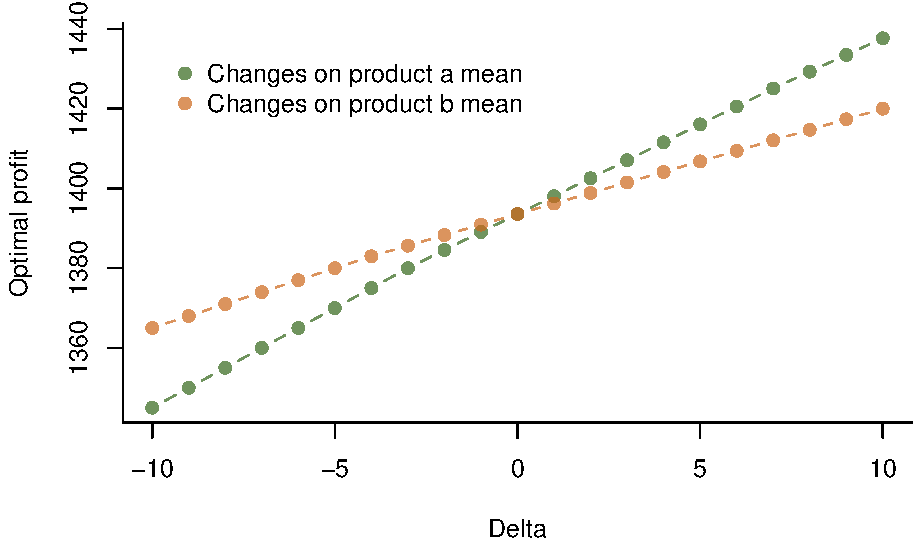
\includegraphics{Example-figure_files/figure-latex/mean-1.pdf}
\label{fig:mean}
\end{figure}

Surprisingly, one may find that increasing mean demand will actually increases manufacturing cost. That is because the ``cost" referred here is ``opportunity cost" \cite{Ch12,Po02}, which is incurred by \emph{not} gaining the benefit associated with the best alternative choice, e.g., the profit could have been earned. As one could notice in sensitivity reports, the time constraint on machine $B$ is binding. Therefore, only promoting mean demand won't bring any gain to the manufacturer, but increases the demand-supply gap, and therefore, increases opportunity cost even more.

Instead, the manufacturer should concentrate on easing the binding constraint, in order to gain more supply power, and therefore meet the demand. Reversely, the manufacturer could also look into anti-promotion methods (if exist), that convert excess demand into cash flow, e.g., ``selling" customer to other manufacturers to get stable cash back.

One can compare these results with simulation outputs in Figure \ref{fig:mean} for verification.

On the other hand, we consider a decrease of standard deviation on estimated demand on product $a$ or $b$. Applying the formulation from subsection \ref{sub:information}, we should have margin gain on decreasing standard deviation by $k\%$ as:
\[
\begin{aligned}
    \Delta \, C_{va} = -12.1 \, k_a,\\
    \Delta \, C_{vb} = -22.1 \, k_b,
\end{aligned}
\]

\begin{figure}[htb]
\centering
\caption{Optimal cost vs. Change of variance}
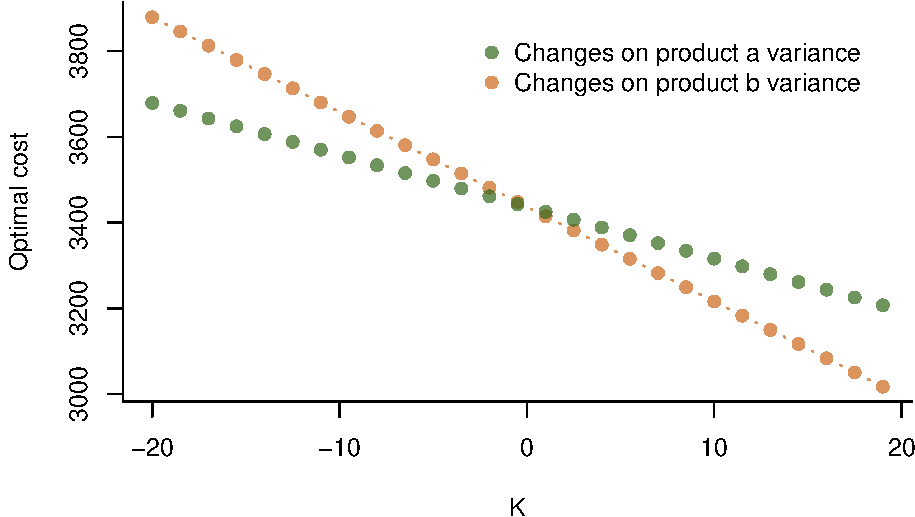
\includegraphics{Example-figure_files/figure-latex/var-1.pdf}
\label{fig:var}
\end{figure}
providing the demand remain positive and variance is no less than zero. In this case, we can see that conducting market research may reduce cost. The simulated results are presented in Figure \ref{fig:var}. The manufacturer, therefore, could decide whether or not to use market research and to what extent should the research be used by comparing research cost and the margin gain.

\section{Experiments}
\label{se:experiment}

In this section, we perform experiments to examine the accuracy and efficiency of the approach.


%%%%%%%%%%%%%%%%%%%%
\section{Summary}
\label{se:conclusion}
This paper provides a framework of applying LP sensitivity analysis on formulated MPNP. Specifically, we use SA technique to estimate the effect of changes in moments of demand distribution on the optimal cost. We first formulate the MPNP into a two-stage stochastic linear programming with recourse, which can be view as large LP model with finite scenarios. Then, we perform the non-standard SA to derive the margin. Therefore, as long as the changes in allowable range, we can inform the market decision directly.

In this paper, we considered two improvements that could alter the demand, each of which was then expressed mathematically. We can, therefore, decide whether to use those effort by comparing the gain and loss.

We also perform an example to demonstrate the approach. The result from our approach is in line with the simulation output.

%%%%%%%%%%%%%%%%%%%%%%%%%%%%%%
\printbibliography
%%%%%%%%%%%%%%%%%%%%%%%%%%%%%%
\newpage
\begin{center}
{\bf\Large Appendices}
\end{center}

\appendix

\section{Sensitivity Report: An Example}
\label{se:report}

\begingroup\fontsize{7}{9}\selectfont
\begin{longtable}{cccccc}
\caption{Sensitivity Report: Variable Cells}
\label{tab:sen_var}\\
\toprule
variable & final value & reduced cost & coefficient & allowable increase & allowable decrease\\
\midrule
\endfirsthead
\multicolumn{6}{@{}l}{\textit{(continued)}}\\
\toprule
variable & final value & reduced cost & coefficient & allowable increase & allowable decrease\\
\midrule
\endhead
\
\endfoot
\bottomrule
\endlastfoot
$y_1^1$ & 7.1 & 0.0 & 5 & 6.0 & 3.8\\
$y_1^2$ & 0.0 & 5.0 & 5 & 10000.0 & 5.0\\
$y_1^3$ & 27.1 & 0.0 & 5 & 6.0 & 3.8\\
$y_1^4$ & 17.1 & 0.0 & 5 & 6.0 & 3.8\\
$y_1^5$ & 17.1 & 0.0 & 5 & 6.0 & 3.8\\
\addlinespace
$y_1^6$ & 0.0 & 5.0 & 5 & 10000.0 & 5.0\\
$y_1^7$ & 0.0 & 5.0 & 5 & 10000.0 & 5.0\\
$y_1^8$ & 0.0 & 5.0 & 5 & 10000.0 & 5.0\\
$y_1^9$ & 7.1 & 0.0 & 5 & 6.0 & 3.8\\
$y_1^{10}$ & 17.1 & 0.0 & 5 & 6.0 & 3.8\\
\addlinespace
$y_1^{11}$ & 0.0 & 5.0 & 5 & 10000.0 & 5.0\\
$y_1^{12}$ & 0.0 & 5.0 & 5 & 10000.0 & 5.0\\
$y_2^1$ & 0.0 & 7.0 & 7 & 10000.0 & 7.0\\
$y_2^2$ & 0.0 & 7.0 & 7 & 10000.0 & 7.0\\
$y_2^3$ & 10.0 & 0.0 & 7 & 2.7 & 4.3\\
\addlinespace
$y_2^4$ & 30.0 & 0.0 & 7 & 2.7 & 4.3\\
$y_2^5$ & 0.0 & 4.3 & 7 & 10000.0 & 4.3\\
$y_2^6$ & 0.0 & 7.0 & 7 & 10000.0 & 7.0\\
$y_2^7$ & 40.0 & 0.0 & 7 & 2.7 & 4.3\\
$y_2^8$ & 60.0 & 0.0 & 7 & 2.7 & 4.3\\
\addlinespace
$y_2^9$ & 30.0 & 0.0 & 7 & 2.7 & 4.3\\
$y_2^{10}$ & 0.0 & 7.0 & 7 & 10000.0 & 7.0\\
$y_2^{11}$ & 0.0 & 7.0 & 7 & 10000.0 & 7.0\\
$y_2^{12}$ & 0.0 & 7.0 & 7 & 10000.0 & 7.0\\
$z_1^1$ & 0.0 & 6.0 & 6 & 10000.0 & 6.0\\
\addlinespace
$z_1^2$ & 12.9 & 0.0 & 6 & 3.8 & 6.0\\
$z_1^3$ & 0.0 & 6.0 & 6 & 10000.0 & 6.0\\
$z_1^4$ & 0.0 & 6.0 & 6 & 10000.0 & 6.0\\
$z_1^5$ & 0.0 & 6.0 & 6 & 10000.0 & 6.0\\
$z_1^6$ & 2.9 & 0.0 & 6 & 3.8 & 6.0\\
\addlinespace
$z_1^7$ & 32.9 & 0.0 & 6 & 3.8 & 6.0\\
$z_1^8$ & 42.9 & 0.0 & 6 & 3.8 & 6.0\\
$z_1^9$ & 0.0 & 6.0 & 6 & 10000.0 & 6.0\\
$z_1^{10}$ & 0.0 & 6.0 & 6 & 10000.0 & 6.0\\
$z_1^{11}$ & 2.9 & 0.0 & 6 & 3.8 & 6.0\\
\addlinespace
$z_1^{12}$ & 32.9 & 0.0 & 6 & 3.8 & 6.0\\
$z_2^1$ & 40.0 & 0.0 & 6 & 4.3 & 2.7\\
$z_2^2$ & 20.0 & 0.0 & 6 & 4.3 & 2.7\\
$z_2^3$ & 0.0 & 6.0 & 6 & 10000.0 & 6.0\\
$z_2^4$ & 0.0 & 6.0 & 6 & 10000.0 & 6.0\\
\addlinespace
$z_2^5$ & 0.0 & 0.0 & 6 & 4.3 & 2.7\\
$z_2^6$ & 0.0 & 0.0 & 6 & 4.3 & 2.7\\
$z_2^7$ & 0.0 & 6.0 & 6 & 10000.0 & 6.0\\
$z_2^8$ & 0.0 & 6.0 & 6 & 10000.0 & 6.0\\
$z_2^9$ & 0.0 & 6.0 & 6 & 10000.0 & 6.0\\
\addlinespace
$z_2^{10}$ & 10.0 & 0.0 & 6 & 4.3 & 2.7\\
$z_2^{11}$ & 50.0 & 0.0 & 6 & 4.3 & 2.7\\
$z_2^{12}$ & 50.0 & 0.0 & 6 & 4.3 & 2.7\\
$x_1$ & 207.1 & 0.0 & 0 & 6.0 & 3.8\\
$x_2$ & 210.0 & 0.0 & 0 & 2.7 & 4.3\\*
\end{longtable}
\endgroup{}

\begingroup\fontsize{6}{9}\selectfont
\begin{longtable}{cccccc}
\caption{Sensitivity Report: Constraints}
\label{tab:sen_con}\\
\toprule
row & final value & shadow price & constraint RHS & allowable increase & allowable decrease\\
\midrule
\endfirsthead
\multicolumn{6}{@{}l}{\textit{(continued)}}\\
\toprule
row & final value & shadow price & constraint RHS & allowable increase & allowable decrease\\
\midrule
\endhead
\
\endfoot
\bottomrule
\endlastfoot
time\_A & 2088.6 & 0.0 & 2200 & 10000.0 & 111.4\\
time\_B & 2500.0 & -0.9 & 2500 & 20.0 & 50.0\\
time\_C & 3337.1 & 0.0 & 3500 & 10000.0 & 162.9\\
over\_1\textasciicircum{}1 & 200.0 & -5.0 & 200 & 7.1 & 10000.0\\
over\_1\textasciicircum{}2 & 207.1 & 0.0 & 220 & 10000.0 & 12.9\\
\addlinespace
over\_1\textasciicircum{}3 & 180.0 & -5.0 & 180 & 27.1 & 10000.0\\
over\_1\textasciicircum{}4 & 190.0 & -5.0 & 190 & 17.1 & 10000.0\\
over\_1\textasciicircum{}5 & 190.0 & -5.0 & 190 & 17.1 & 10000.0\\
over\_1\textasciicircum{}6 & 207.1 & 0.0 & 210 & 10000.0 & 2.9\\
over\_1\textasciicircum{}7 & 207.1 & 0.0 & 240 & 10000.0 & 32.9\\
\addlinespace
over\_1\textasciicircum{}8 & 207.1 & 0.0 & 250 & 10000.0 & 42.9\\
over\_1\textasciicircum{}9 & 200.0 & -5.0 & 200 & 7.1 & 10000.0\\
over\_1\textasciicircum{}10 & 190.0 & -5.0 & 190 & 17.1 & 10000.0\\
over\_1\textasciicircum{}11 & 207.1 & 0.0 & 210 & 10000.0 & 2.9\\
over\_1\textasciicircum{}12 & 207.1 & 0.0 & 240 & 10000.0 & 32.9\\
\addlinespace
under\_1\textasciicircum{}1 & 207.1 & 0.0 & 200 & 7.1 & 10000.0\\
under\_1\textasciicircum{}2 & 220.0 & 6.0 & 220 & 10000.0 & 12.9\\
under\_1\textasciicircum{}3 & 207.1 & 0.0 & 180 & 27.1 & 10000.0\\
under\_1\textasciicircum{}4 & 207.1 & 0.0 & 190 & 17.1 & 10000.0\\
under\_1\textasciicircum{}5 & 207.1 & 0.0 & 190 & 17.1 & 10000.0\\
\addlinespace
under\_1\textasciicircum{}6 & 210.0 & 6.0 & 210 & 10000.0 & 2.9\\
under\_1\textasciicircum{}7 & 240.0 & 6.0 & 240 & 10000.0 & 32.9\\
under\_1\textasciicircum{}8 & 250.0 & 6.0 & 250 & 10000.0 & 42.9\\
under\_1\textasciicircum{}9 & 207.1 & 0.0 & 200 & 7.1 & 10000.0\\
under\_1\textasciicircum{}10 & 207.1 & 0.0 & 190 & 17.1 & 10000.0\\
\addlinespace
under\_1\textasciicircum{}11 & 210.0 & 6.0 & 210 & 10000.0 & 2.9\\
under\_1\textasciicircum{}12 & 240.0 & 6.0 & 240 & 10000.0 & 32.9\\
over\_2\textasciicircum{}1 & 210.0 & 0.0 & 250 & 10000.0 & 40.0\\
over\_2\textasciicircum{}2 & 210.0 & 0.0 & 230 & 10000.0 & 20.0\\
over\_2\textasciicircum{}3 & 200.0 & -7.0 & 200 & 10.0 & 10000.0\\
\addlinespace
over\_2\textasciicircum{}4 & 180.0 & -7.0 & 180 & 30.0 & 10000.0\\
over\_2\textasciicircum{}5 & 210.0 & -2.7 & 210 & 0.0 & 4.0\\
over\_2\textasciicircum{}6 & 210.0 & 0.0 & 210 & 10000.0 & 0.0\\
over\_2\textasciicircum{}7 & 170.0 & -7.0 & 170 & 40.0 & 10000.0\\
over\_2\textasciicircum{}8 & 150.0 & -7.0 & 150 & 60.0 & 10000.0\\
\addlinespace
over\_2\textasciicircum{}9 & 180.0 & -7.0 & 180 & 30.0 & 10000.0\\
over\_2\textasciicircum{}10 & 210.0 & 0.0 & 220 & 10000.0 & 10.0\\
over\_2\textasciicircum{}11 & 210.0 & 0.0 & 260 & 10000.0 & 50.0\\
over\_2\textasciicircum{}12 & 210.0 & 0.0 & 260 & 10000.0 & 50.0\\
under\_2\textasciicircum{}1 & 250.0 & 6.0 & 250 & 10000.0 & 40.0\\
\addlinespace
under\_2\textasciicircum{}2 & 230.0 & 6.0 & 230 & 10000.0 & 20.0\\
under\_2\textasciicircum{}3 & 210.0 & 0.0 & 200 & 10.0 & 10000.0\\
under\_2\textasciicircum{}4 & 210.0 & 0.0 & 180 & 30.0 & 10000.0\\
under\_2\textasciicircum{}5 & 210.0 & 6.0 & 210 & 10000.0 & 0.0\\
under\_2\textasciicircum{}6 & 210.0 & 6.0 & 210 & 10000.0 & 0.0\\
\addlinespace
under\_2\textasciicircum{}7 & 210.0 & 0.0 & 170 & 40.0 & 10000.0\\
under\_2\textasciicircum{}8 & 210.0 & 0.0 & 150 & 60.0 & 10000.0\\
under\_2\textasciicircum{}9 & 210.0 & 0.0 & 180 & 30.0 & 10000.0\\
under\_2\textasciicircum{}10 & 220.0 & 6.0 & 220 & 10000.0 & 10.0\\
under\_2\textasciicircum{}11 & 260.0 & 6.0 & 260 & 10000.0 & 50.0\\
\addlinespace
under\_2\textasciicircum{}12 & 260.0 & 6.0 & 260 & 10000.0 & 50.0\\*
\end{longtable}
\endgroup{}



\end{document}
